\documentclass[12pt]{scrartcl}

\usepackage{amsmath,amssymb}
\usepackage{fullpage}
\usepackage{enumitem}
\usepackage{hyperref}
\usepackage{listings}
\usepackage{xcolor}

% Tables/figures/diagrams
\usepackage{graphicx}
\usepackage{booktabs}
\usepackage{array}
\usepackage{caption}
\usepackage{tikz}
\usetikzlibrary{arrows.meta,positioning,calc}

\setlength{\parindent}{0pt}

\lstset{
    language=Python,
    basicstyle=\ttfamily\small,
    keywordstyle=\color{blue},
    commentstyle=\color{gray},
    stringstyle=\color{teal},
    frame=single,
    columns=fullflexible,
    keepspaces=true,
    showstringspaces=false
}

\begin{document}

% \begin{center}
% 	\hrule
% 	\vspace{0.4cm}
% 	{\textbf{\large Tutorial 02}}\\[0.2cm]
% 	INF1008 Data Structures and Algorithms
% \end{center}

% \textbf{Name:} Timothy Chia\hspace{\fill} \textbf{Student ID:} 2501530\\

% \hrule

% \vspace{0.3cm}

\section*{Lecture 02: Analysis of Algorithms}
INF1008 Data Structures and Algorithms \\
Written By: Timothy Chia

\vspace{0.2cm}
\tableofcontents
\vspace{0.2cm}

\newpage
\section{Introduction to Algorithm Analysis}
An \textbf{algorithm} is a finite, unambiguous sequence of steps that transforms an \emph{input} into an \emph{output} and is guaranteed to terminate. In computing, correctness is only the first requirement. We also care about \emph{efficiency}: whether the algorithm remains usable when the input becomes large.

Algorithm analysis answers questions such as:
\begin{itemize}[leftmargin=1.5em]
	\item If the input size doubles, does the running time roughly double, quadruple, or become completely infeasible?
	\item Is the algorithm limited by \emph{time} (too slow) or \emph{space} (uses too much memory)?
\end{itemize}

\textbf{Time complexity} describes how the running time grows with the input size \(n\). \textbf{Space complexity} describes how memory usage grows with \(n\). The goal is not to predict the exact number of milliseconds on one machine, but to understand \emph{scalability}. Small constant differences matter for tiny inputs; growth rates dominate for large inputs.

A useful mindset is: \emph{efficiency is about the shape of growth}. This is why we develop mathematical tools to count how often key operations run as \(n\) increases.

\subsection{Order of Growth}
Order of growth compares how resources scale as the \emph{volume} of input grows. A simple way to build intuition is to contrast a \emph{bundled} process that has a fixed overhead with a \emph{per-item} process whose cost increases with the number of items. For instance, suppose a bundled method takes a fixed \(24\) hours regardless of how many items are requested, while a per-item method takes about \(2\) hours per item, giving \(T(n)=2n\) hours. The exact numbers are not the point; the growth pattern is. When \(n\) doubles, the bundled time stays the same, while the per-item time doubles.

\begin{figure}[h]
	\centering
	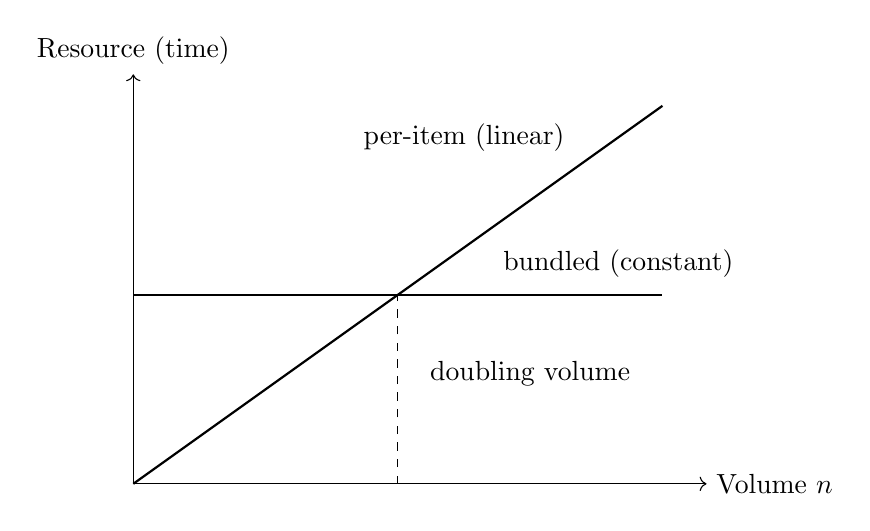
\begin{tikzpicture}[x=0.28cm,y=0.10cm]
		\draw[->] (0,0) -- (26,0) node[right] {Volume \(n\)};
		\draw[->] (0,0) -- (0,52) node[above] {Resource (time)};
		\draw[thick] plot[domain=0:24] (\x,{24});
		\node[align=left] at (22,28) {bundled\ (constant)};
		\draw[thick] plot[domain=0:24] (\x,{2*\x});
		\node[align=left] at (15,44) {per-item\ (linear)};
		\draw[dashed] (12,0) -- (12,24) -- (0,24);
		\node[draw=none, align=left] at (18,14) {doubling\ volume};
	\end{tikzpicture}
	\caption{Constant vs linear growth: the bundled method is \(O(1)\) in volume; the per-item method is \(O(n)\).}
\end{figure}

\section{Mathematics for Algorithms}
This section collects the core mathematical ideas used to analyse loops and recursion. Each concept will reappear later when we count operations and simplify complexity expressions.

\subsection{Polynomials and dominance of the highest-degree term}
A polynomial has the form
\[
	p(n)=a_dn^d+a_{d-1}n^{d-1}+\cdots+a_1n+a_0,
\]
where \(d\) is the degree and \(a_d\neq 0\). For large \(n\), the term \(a_dn^d\) dominates the growth because \(n^d\) eventually overwhelms every lower power.

To see this, divide by the highest power:
\[
	\frac{p(n)}{n^d}=a_d+\frac{a_{d-1}}{n}+\cdots+\frac{a_0}{n^d}\xrightarrow[n\to\infty]{}a_d.
\]
So, for large \(n\), \(p(n)\) behaves like \(a_dn^d\) up to constant factors.

\begin{table}[h]
	\centering
	\caption{Dominant-term intuition for common polynomials.}
	\begin{tabular}{@{}>{\raggedright}p{0.52\textwidth} >{\raggedright}p{0.40\textwidth}@{}}
		\toprule
		Polynomial \(p(n)\) & Dominant behaviour as \(n\) grows \\ \midrule
		\(3n+7\)            & behaves like \(n\) (linear)       \\
		\(2n^2+3n+3\)       & behaves like \(n^2\) (quadratic)  \\
		\(n^3+100n^2+7\)    & behaves like \(n^3\) (cubic)      \\
		\(5n^4 + n\)        & behaves like \(n^4\) (quartic)    \\
		\bottomrule
	\end{tabular}
\end{table}

\subsection{Combinations and loop counting (1-Sum and 2-Sum)}
A \textbf{combination} counts ways to choose \(k\) items from \(n\) items without caring about order:
\[
	\binom{n}{k}=\frac{n!}{k!(n-k)!}.
\]
This connects naturally to algorithms that examine all pairs, triples, or subsets of elements.

\paragraph{1-Sum (single loop).}
If a loop performs constant work once per iteration from \(1\) to \(n\), the total work is
\[
	\sum_{i=1}^{n} 1 = n.
\]
The key idea: one loop with \(n\) iterations typically gives linear growth.

\paragraph{2-Sum (triangular nested loop).}
A common nested-loop pattern is:
\begin{lstlisting}
for i in range(1, n+1):
    for j in range(i+1, n+1):
        # constant work
        pass
\end{lstlisting}

For each fixed \(i\), the inner loop runs \(n-i\) times. Total inner executions:
\begin{align*}
	\sum_{i=1}^{n} (n-i) & = (n-1)+(n-2)+\cdots+1 \\
	                     & =\frac{n(n-1)}{2}      \\
	                     & =\binom{n}{2}.
\end{align*}
This triangular count is the reason ``all-pairs'' style algorithms are typically quadratic.

\begin{figure}[h]
	\centering
	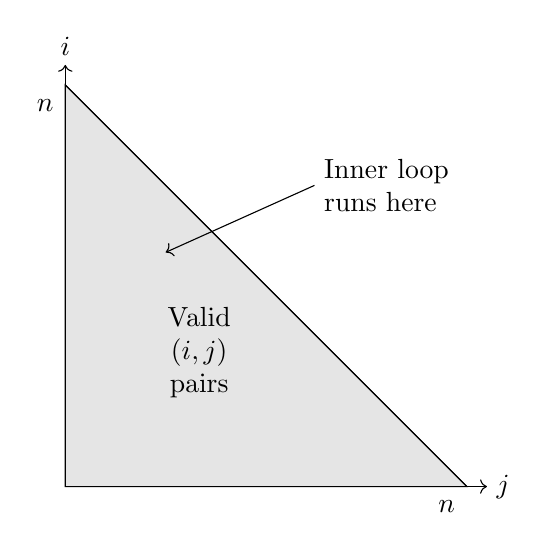
\begin{tikzpicture}[scale=0.85]
		\draw[->] (0,0) -- (6.3,0) node[right] {$j$};
		\draw[->] (0,0) -- (0,6.3) node[above] {$i$};
		\draw (0,6) -- (6,0);
		\draw[fill=black!10] (0,0) -- (0,6) -- (6,0) -- cycle;

		\node[align=center] at (2.0,2.0) {Valid\\\((i,j)\)\\pairs};

		% Text outside + arrow into the shaded region
		\node[align=left] (innerlabel) at (4.8,4.5) {Inner loop\\runs here};
		\draw[->] (innerlabel.west) -- (1.5,3.5);

		\node at (5.7,-0.3) {$n$};
		\node at (-0.3,5.7) {$n$};
	\end{tikzpicture}
	\caption{The 2-Sum nested loop counts a triangular region of index pairs, giving \(\frac{n(n-1)}{2}\) inner executions.}
\end{figure}

\subsection{Logarithms and repeated halving}
A logarithm answers: ``what exponent produces \(n\)?''
\[
	\log_b(n)=x \iff b^x=n,\quad b>0,\ b\neq 1,\ n>0.
\]
Logarithms appear whenever an algorithm repeatedly \emph{halves} (or, more generally, divides by a constant factor) the problem size.

\paragraph{Repeated halving.}
Suppose you start with \(n\) and keep dividing by 2 until reaching 1:
\[
	n,\ \frac{n}{2},\ \frac{n}{4},\ \dots,\ 1.
\]
After \(k\) steps you have \(n/2^k\). Set \(n/2^k=1\) to get \(2^k=n\), so \(k=\log_2 n\). This is why binary search runs in \(O(\log n)\): each step removes about half the remaining candidates.

\begin{table}[h]
	\centering
	\caption{Useful logarithm laws for simplifying runtime expressions.}
	\begin{tabular}{@{}p{0.35\textwidth} p{0.55\textwidth}@{}}
		\toprule
		Law                                       & Meaning                                       \\ \midrule
		\(\log_b(xy)=\log_b x+\log_b y\)          & products become sums                          \\
		\(\log_b(x/y)=\log_b x-\log_b y\)         & quotients become differences                  \\
		\(\log_b(x^k)=k\log_b x\)                 & exponents become multipliers                  \\
		\(\log_a n = \dfrac{\log_b n}{\log_b a}\) & change of base (differs by a constant factor) \\
		\bottomrule
	\end{tabular}
\end{table}

\begin{figure}[h]
	\centering
	\begin{tikzpicture}[node distance=1.5cm, every node/.style={draw, rounded corners, align=center}]
		\node (n0) {$n$ items};
		\node (n1) [below=of n0] {$n/2$ items};
		\node (n2) [below=of n1] {$n/4$ items};
		\node (n3) [below=of n2] {$\vdots$};
		\node (n4) [below=of n3] {$1$ item};

		\draw[-{Stealth}] (n0) -- (n1) node[midway, right, draw=none] {halve};
		\draw[-{Stealth}] (n1) -- (n2) node[midway, right, draw=none] {halve};
		\draw[-{Stealth}] (n2) -- (n3);
		\draw[-{Stealth}] (n3) -- (n4);

		\node[draw=none, right=3.5cm of n2, align=left] (note) {Number of halving steps\\to reach \(1\) is\\\(\log_2 n\).};
		\draw[-{Stealth}] (note.west) -- (n2.east);
	\end{tikzpicture}
	\caption{Repeated halving leads to logarithmic time.}
\end{figure}

\newpage
\subsection{Summation of series and algorithm costs}
Many runtimes are expressed as summations, especially when counting loop iterations.

\paragraph{Arithmetic series.}
\[
	\sum_{i=1}^{n} i = \frac{n(n+1)}{2}.
\]
This is the mathematical reason triangular nested loops often yield quadratic growth.

\paragraph{Geometric series.}
For ratio \(r\neq 1\),
\[
	\sum_{i=0}^{k} r^i=\frac{r^{k+1}-1}{r-1}.
\]
When \(r=2\), \(1+2+4+\cdots+2^k=2^{k+1}-1\). Geometric sums frequently appear in divide-and-conquer recurrences and in processes that repeatedly double/halve.

\begin{table}[h]
	\centering
	\caption{Series formulas that commonly appear in loop and recursion analysis.}
	\begin{tabular}{@{}p{0.46\textwidth} p{0.46\textwidth}@{}}
		\toprule
		Series                            & Closed form               \\ \midrule
		\(\sum_{i=1}^{n} 1\)              & \(n\)                     \\
		\(\sum_{i=1}^{n} i\)              & \(\frac{n(n+1)}{2}\)      \\
		\(\sum_{i=0}^{k} r^i\ (r\neq 1)\) & \(\frac{r^{k+1}-1}{r-1}\) \\
		\(\sum_{i=0}^{k} 2^i\)            & \(2^{k+1}-1\)             \\
		\bottomrule
	\end{tabular}
\end{table}

\section{Empirical vs Theoretical Analysis}
There are two broad ways to evaluate an algorithm.\\ [0.2cm]
Empirical analysis measures time and memory by running real code on a real system. This is excellent for engineering decisions (choice of language, data layout, constant-factor improvements), but it is difficult to generalise. Measurements depend on CPU speed, caching, compiler optimisations, the operating system, background processes, and the input distribution. \\ [0.2cm]
Theoretical analysis uses a simplified computational model and counts abstract operations as a function of input size \(n\). The advantage is portability: the result is a machine-independent prediction of scalability. Theoretical models are especially valuable when inputs can grow far beyond what is comfortable to benchmark.

\begin{table}[h]
	\centering
	\caption{Empirical vs theoretical analysis: what each approach tells you.}
	\begin{tabular}{@{}p{0.46\textwidth} p{0.46\textwidth}@{}}
		\toprule
		Empirical (measurements)                 & Theoretical (models)                         \\ \midrule
		Depends on hardware/software settings    & Independent of specific machines             \\
		Captures constant factors and overhead   & Focuses on growth rates                      \\
		Requires implementation and testing      & Enables early comparison before coding       \\
		Sensitive to input distribution used     & Usually analyses worst-case or general \(n\) \\
		Best for optimisation \emph{in practice} & Best for predicting \emph{scalability}       \\
		\bottomrule
	\end{tabular}
\end{table}

\newpage
\section{Computational Models}
To analyse algorithms theoretically, we need a model of what counts as ``work''.

\subsection{RAM model}
The \textbf{RAM model} assumes:
\begin{enumerate}[leftmargin=1.5em]
	\item Each elementary operation takes constant time.
	\item Accessing any memory location takes constant time.
	\item The cost of an algorithm is approximated by counting elementary operations.
\end{enumerate}

Under this model, operations such as assignment, arithmetic, comparisons, and array indexing are treated as constant time.

\begin{table}[h]
	\centering
	\caption{Examples of elementary operations (each treated as \(O(1)\) in the RAM model).}
	\begin{tabular}{@{}p{0.35\textwidth} p{0.55\textwidth}@{}}
		\toprule
		Category        & Examples                                                    \\ \midrule
		Arithmetic      & \(+,-,\times,\div\) on fixed-size numbers                   \\
		Assignment      & \(x \leftarrow y\), \(x \leftarrow c\)                      \\
		Comparison      & \(x<y\), \(x==y\)                                           \\
		Logic/branching & \texttt{if}, \texttt{else}, \texttt{while} condition checks \\
		Memory access   & reading/writing \(A[i]\)                                    \\
		\bottomrule
	\end{tabular}
\end{table}

\subsection{Operation counting with 1-Sum and 2-Sum}
Operation counting converts code into a cost function \(T(n)\). A consistent method is:
\begin{enumerate}[leftmargin=1.5em]
	\item Identify the input size \(n\).
	\item Choose which statements count as unit-cost operations.
	\item Count how often each statement executes.
	\item Sum the contributions to obtain \(T(n)\), then simplify.
\end{enumerate}

\paragraph{Example: 1-Sum.}
Consider:
\begin{lstlisting}
def one_sum(A):
    s = 0
    for i in range(len(A)):
        s += A[i]
    return s
\end{lstlisting}

If we count a constant number of operations per loop iteration, the total is of the form
\[
	T(n)=an+b,
\]
for some constants \(a,b>0\). This is linear growth: doubling \(n\) roughly doubles \(T(n)\).

\paragraph{Example: counting an iterative factorial.}
Consider:
\begin{lstlisting}
def factorial(n):
    res, val = 1, 1
    while val <= n:
        res = res * val
        val = val + 1
    return res
\end{lstlisting}

If we treat assignment, comparison, addition, and multiplication as unit-cost steps, then each loop iteration performs a constant number of such steps. The loop runs \(n\) times (plus one final condition check), so the total cost is linear: \(T(n)=an+b\) for constants \(a,b>0\), hence \(T(n)=O(n)\).

\begin{table}[h]
	\centering
	\caption{Illustrative step count for iterative factorial under a simple unit-cost model.}
	\begin{tabular}{@{}c c c@{}}
		\toprule
		\(n\) & steps \(T(n)\) (example) & growth        \\ \midrule
		1     & \(5(1)+4=9\)             &               \\
		2     & \(5(2)+4=14\)            &               \\
		3     & \(5(3)+4=19\)            & \(\propto n\) \\
		4     & \(5(4)+4=24\)            &               \\ \bottomrule
	\end{tabular}
\end{table}

\paragraph{Example: 2-Sum.}
Consider:
\begin{lstlisting}
def two_sum(A):
    s = 0
    n = len(A)
    for i in range(n):
        for j in range(i+1, n):
            s += A[i] + A[j]
    return s
\end{lstlisting}

The inner loop runs \((n-1)+(n-2)+\cdots+1=\frac{n(n-1)}{2}\) times. If each inner iteration performs constant work, then the dominant term of \(T(n)\) is proportional to \(n^2\).

\begin{table}[h]
	\centering
	\caption{Counting inner-loop executions for the 2-Sum pattern.}
	\begin{tabular}{@{}c c c@{}}
		\toprule
		Outer index \(i\) & Inner iterations \(n-i-1\) & Contribution                                  \\ \midrule
		\(0\)             & \(n-1\)                    & \(n-1\)                                       \\
		\(1\)             & \(n-2\)                    & \(n-2\)                                       \\
		\(\vdots\)        & \(\vdots\)                 & \(\vdots\)                                    \\
		\(n-2\)           & \(1\)                      & \(1\)                                         \\
		\(n-1\)           & \(0\)                      & \(0\)                                         \\ \midrule
		Total             &                            & \(\sum_{i=0}^{n-1} (n-i-1)=\frac{n(n-1)}{2}\) \\
		\bottomrule
	\end{tabular}
\end{table}


\section{Asymptotic Analysis}
Exact counts (like \(3n+3\) or \(2n^2+3n+3\)) are useful, but algorithm comparison is usually driven by how \(T(n)\) grows for large \(n\). \textbf{Asymptotic analysis} describes growth while ignoring constant factors and lower-order terms.

\subsection{Motivation: growth for large inputs and worst-case focus}
As \(n\) grows, the dominant term decides feasibility. For example, \(n^2\) grows faster than \(n\log n\), and both grow far slower than \(2^n\). This is why we focus on large-input behaviour rather than small-input timing.

Worst-case analysis is commonly used because it provides a performance guarantee: for inputs of size \(n\), the algorithm will not exceed the derived upper bound.

\subsection{Big-O: formal definition and intuition}
\textbf{Big-O} provides an asymptotic upper bound.

\[
	f(n)=O(g(n)) \iff \exists\,k>0,\ \exists\,n_0\ \text{s.t.}\ \forall n\ge n_0,\ f(n)\le k\,g(n).
\]

Intuitively, once \(n\) is large enough, \(g(n)\) (up to a constant multiple) sits above \(f(n)\).

\paragraph{Worked proof (1-Sum).}
Let \(f(n)=3n+3\). We show \(f(n)=O(n)\). For \(n\ge 1\), \(3\le 3n\), so
\[
	3n+3 \le 3n+3n = 6n.
\]
Choose \(k=6\) and \(n_0=1\). Then \(f(n)\le k n\) for all \(n\ge n_0\), hence \(3n+3=O(n)\).

\paragraph{Worked proof (2-Sum).}
Let \(f(n)=2n^2+3n+3\). We show \(f(n)=O(n^2)\). For \(n\ge 1\), \(3n\le 3n^2\) and \(3\le 3n^2\), so
\[
	2n^2+3n+3 \le 2n^2 + 3n^2 + 3n^2 = 8n^2.
\]
Choose \(k=8\) and \(n_0=1\). Then \(f(n)\le k n^2\) for all \(n\ge n_0\), hence \(f(n)=O(n^2)\).

\subsection{Big-Omega and Big-Theta}
\textbf{Big-Omega} is an asymptotic lower bound:
\[
	f(n)=\Omega(g(n)) \iff \exists\,k>0,\ \exists\,n_0\ \text{s.t.}\ \forall n\ge n_0,\ f(n)\ge k\,g(n).
\]

\textbf{Big-Theta} is a tight bound (both upper and lower):
\[
	f(n)=\Theta(g(n)) \iff f(n)=O(g(n))\ \text{and}\ f(n)=\Omega(g(n)).
\]

\paragraph{Interpretation.}
If \(T(n)=O(g(n))\), the algorithm grows no faster than \(g(n)\) up to constants. If \(T(n)=\Omega(g(n))\), it grows at least as fast as \(g(n)\). If \(T(n)=\Theta(g(n))\), then \(g(n)\) captures the true growth rate (within constant factors).

\begin{figure}[h]
	\centering
	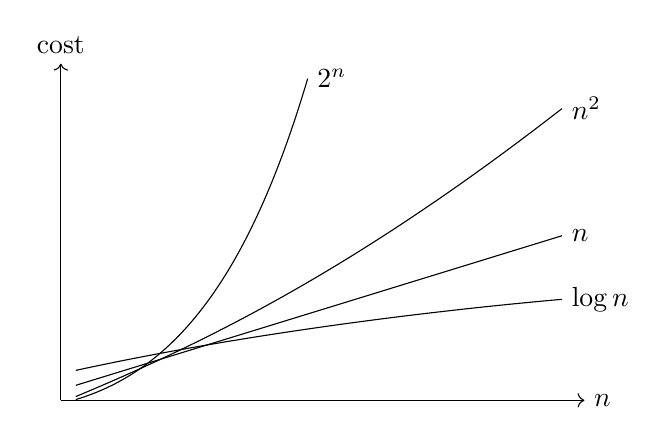
\begin{tikzpicture}[scale=0.95]
		\draw[->] (0,0) -- (7,0) node[right] {$n$};
		\draw[->] (0,0) -- (0,4.5) node[above] {cost};

		% Curves (qualitative)
		\draw (0.2,0.4) .. controls (2.5,0.9) and (5,1.2) .. (6.7,1.35) node[right] {$\log n$};
		\draw (0.2,0.2) -- (6.7,2.2) node[right] {$n$};
		\draw (0.2,0.05) .. controls (2,0.8) and (4,1.8) .. (6.7,3.9) node[right] {$n^2$};
		\draw (0.2,0.01) .. controls (1.5,0.4) and (2.5,1.6) .. (3.3,4.3) node[right] {$2^n$};

		% \node[align=left] at (4.2,0.55) {Curves are\\not to scale;\\they show\\relative growth.};
	\end{tikzpicture}
	\caption{Qualitative growth-rate comparison: logarithmic \(\ll\) linear \(\ll\) quadratic \(\ll\) exponential.}
\end{figure}

\section{Combining and Simplifying Growth}
Real algorithms combine multiple parts. To compute a clean asymptotic bound, we use a small set of rules.

\subsection{Sequential components}
If an algorithm runs part A then part B, the total time is
\[
	T(n)=T_A(n)+T_B(n).
\]
As \(n\) grows, the dominant term determines the final class. For example, \(n^2 + 10n\) behaves like \(n^2\).

\subsection{Nested components}
If a loop of \(n\) iterations contains an inner process of cost \(T_{\text{inner}}(n)\), the total often multiplies:
\[
	T(n)=n\cdot T_{\text{inner}}(n).
\]
For example, an outer loop \(n\) times and an inner loop \(n\) times gives \(n\cdot n = n^2\).

\subsection{Dominant term analysis}
Two simplifications are standard:
\begin{enumerate}[leftmargin=1.5em]
	\item \textbf{Ignore constant factors:} \(c\cdot g(n)\) is the same growth class as \(g(n)\) for any constant \(c>0\).
	\item \textbf{Ignore lower-order terms:} when adding terms, keep only the fastest-growing term.
\end{enumerate}

So \(2n^2 + 3n + 3\) simplifies to \(\Theta(n^2)\). This is not claiming constants are meaningless; it is claiming they do not change the growth family.

\section{Common Orders of Growth}
The most common growth classes appear across sorting, searching, graph algorithms, and dynamic programming.

\begin{table}[h]
	\centering
	\caption{Common orders of growth with intuition and typical examples.}
	\begin{tabular}{@{}p{0.13\textwidth} p{0.18\textwidth} p{0.29\textwidth} p{0.30\textwidth}@{}}
		\toprule
		Class          & Name         & Typical pattern                                  & Scaling intuition                                 \\ \midrule
		\(O(1)\)       & constant     & array index access, hash lookup (idealised)      & cost unchanged as \(n\) grows                     \\
		\(O(\log n)\)  & logarithmic  & binary search, balanced BST operations           & each step halves remaining work                   \\
		\(O(n)\)       & linear       & scanning a list, finding max                     & one pass over the data                            \\
		\(O(n\log n)\) & linearithmic & merge sort, heapsort                             & \(\log n\) levels \(\times\) \(n\) work per level \\
		\(O(n^2)\)     & quadratic    & all pairs, simple nested loops                   & work for every pair of items                      \\
		\(O(n^3)\)     & cubic        & triple nested loops, naive matrix multiplication & work for every triple                             \\
		\(O(2^n)\)     & exponential  & brute force over all subsets                     & doubling \(n\) squares the search space size      \\ \bottomrule
	\end{tabular}
\end{table}

A helpful practical perspective is: \(O(n)\) and \(O(n\log n)\) often scale well; \(O(n^2)\) becomes heavy when \(n\) is large; exponential growth becomes infeasible extremely quickly.

\section{Types of Algorithm Analysis}
An algorithm can behave differently depending on the input. Therefore, analysis often considers multiple cases:

\textbf{Best-case} is the minimum running time over all inputs of size \(n\). \textbf{Worst-case} is the maximum. \textbf{Average-case} is the expected running time under an assumed probability distribution over inputs.

Worst-case analysis is commonly used because it provides a reliable guarantee, especially when inputs are unpredictable or adversarial.

\begin{table}[h]
	\centering
	\caption{Best-, average-, and worst-case illustrated with a simple search task.}
	\begin{tabular}{@{}p{0.18\textwidth} p{0.74\textwidth}@{}}
		\toprule
		Case         & Example: linear search for a target in an array of length \(n\)                                                       \\ \midrule
		Best-case    & target is at the first position \(\Rightarrow\) 1 comparison \(\Rightarrow O(1)\)                                     \\
		Average-case & target is equally likely to be in any position \(\Rightarrow\) about \(\frac{n}{2}\) comparisons \(\Rightarrow O(n)\) \\
		Worst-case   & target is absent or at the last position \(\Rightarrow\) \(n\) comparisons \(\Rightarrow O(n)\)                       \\
		\bottomrule
	\end{tabular}
\end{table}

Different algorithms can have the same worst-case class but different practical behaviour; likewise, some algorithms have excellent average-case performance yet poor worst-case guarantees. In a first analysis, worst-case bounds are the standard baseline.

\section{Theory of Algorithms}
Algorithm theory connects \emph{what is achievable} with \emph{what is optimal}. Two ideas are central:

\paragraph{Upper bounds.}
An algorithm has an upper bound \(O(g(n))\) if we can prove it never grows faster than \(g(n)\) (up to constants) for sufficiently large \(n\).

\paragraph{Lower bounds.}
A problem has a lower bound \(\Omega(h(n))\) under a given computational model if no algorithm can solve the problem asymptotically faster than \(h(n)\) in the worst case.

\paragraph{Optimal algorithms.}
An algorithm is \textbf{asymptotically optimal} (for a model and problem) if its upper bound matches a proven lower bound up to constant factors, i.e.\ it achieves \(\Theta(\cdot)\) equal to the lower bound. This matters because it tells you when further improvement requires changing assumptions (e.g.\ randomness, extra memory, approximation) rather than simply ``coding better''.

\paragraph{From theory to practice.}
In real systems, you still care about constants, memory limits, and typical inputs. However, asymptotic bounds remain the first filter for selecting algorithms that will not collapse when data grows. Once you have the right growth class, implementation details and empirical testing become the next step for performance tuning.

\end{document}
